%%%%%%%%%%%%%%%%%%%%%%%%%%%%%%%%%%%%%%%%%%%%%%%%%%%%%%%%%%%%%%
\section{Métodos Numéricos}
%%%%%%%%%%%%%%%%%%%%%%%%%%%%%%%%%%%%%%%%%%%%%%%%%%%%%%%%%%%%%%

%%%%%%%%%%%%%%%%%%%%%%%%%%%%%%%%%%%%%%%%%%%%%%%%%%%%%%%%%%%%%%
\subsection{Discretização temporal e espacial}
%%%%%%%%%%%%%%%%%%%%%%%%%%%%%%%%%%%%%%%%%%%%%%%%%%%%%%%%%%%%%%

%%%%%%%%%%%%%%%%%%%%%%%%%%%%%%%%%%%%%%%%%%%%%%%%%%%%%%%%%%%%%%
\begin{frame}{Runge-Kutta}
Para realizar o avanço temporal, envolvendo as Equações \eqref{eq_conservacao_momentum_nao_newtoniano_admensional} e \eqref{eq_tensores_lpog_admensional}, utiliza-se o método de Runge-Kutta de quarta ordem de precisão \cite{ferziger2002computational}. Os quatro passos do método são descritos pelas seguintes equações:
\begin{gather}
    \begin{aligned}
        &\textbf{1º passo:}& \hspace{0.3cm}\varphi^{\left(n+\frac{1}{2}\right)^{*}} &= \varphi^n+\frac{\Delta t}{2} g_{\varphi}\left(t^n, \varphi^n\right),\\
        &\textbf{2º passo:}& \hspace{0.3cm}\varphi^{\left(n+\frac{1}{2}\right)^{* *}} &= \varphi^n+\frac{\Delta t}{2} g_{\varphi}\left(t^{n+\frac{1}{2}}, \varphi^{\left(n+\frac{1}{2}\right)^*}\right),\\
        &\textbf{3º passo:}& \hspace{0.3cm}\varphi^{(n+1)^*} &= \varphi^n+\Delta t g_{\varphi}\left(t^{n+\frac{1}{2}},\varphi^{\left(n+\frac{1}{2}\right)^{* *}}\right),\\
        &\textbf{4º passo:}& \hspace{0.3cm}\varphi^{n+1} &= \varphi^n+\frac{\Delta t}{6}\bigg[g_{\varphi}\left(t^n, \varphi^n\right) + 2 g_{\varphi}\left(t^{n+\frac{1}{2}}, \varphi^{\left(n+\frac{1}{2}\right)^{*}}\right) + \\
        & & & ~~~ + 2 g_{\varphi}\left(t^{n+\frac{1}{2}}, \varphi_{z}^{\left(n+\frac{1}{2}\right)^{**}}\right)+ g_{\varphi}\left(t^{n+1}, \varphi^{(n+1)^{*}}\right)\bigg].\label{eq_rk_4order}
    \end{aligned}
\end{gather}
\end{frame}

%%%%%%%%%%%%%%%%%%%%%%%%%%%%%%%%%%%%%%%%%%%%%%%%%%%%%%%%%%%%%%
\begin{frame}{Runge-Kutta}
No método de Runge-Kutta $\varphi$ descritos em \ref{eq_rk_4order} representa as funções $\omega_{z}$, $T_{xx}$, $T_{xy}$ ou $T_{yy}$. Para a vorticidade $\omega_{z}$, a expressão de $g_{\omega_{z}}(t, \omega_{z})$ é dada como segue:
\begin{gather}
    \begin{aligned}
        g_{\omega_{z}}\left(t, \omega_z\right) = &~- u\frac{\partial\left(\omega_{z}\right)}{\partial x} - v \frac{\partial\left(\omega_{z}\right)}{\partial y} + \frac{\beta_{nn}}{R e}\left(\frac{\partial^2 \omega_{z}}{\partial x^2} + \frac{\partial^2 \omega_{z}}{\partial y^2}\right) + \frac{\partial^2 T_{x x}}{\partial x \partial y} + \frac{\partial^2 T_{x y}}{\partial y^2} - \\ &~- \frac{\partial^2 T_{x y}}{\partial x^2} - \frac{\partial^2 T_{y y}}{\partial x \partial y},
    \end{aligned}
\end{gather}
Para os tensores $T_{xx}$, $T_{xy}$ e $T_{yy}$, as expressões correspondentes são as seguintes:
\begin{gather}
    \begin{aligned}
        g_{T_{xx}}\left(t, T_{xx}\right) = &~- \frac{f(\mathbf{T})T_{xx}}{\operatorname{Wi}} - \left[\frac{\partial (uT_{xx})}{\partial x} + \frac{\partial (vT_{xx})}{\partial y} - 2T_{xx}\frac{\partial u}{\partial x} - 2T_{xy}\frac{\partial u}{\partial y}\right] - \\ &~- \frac{\alpha_{G}\operatorname{Re}}{1-\beta_{nn}}\left(T_{xx}^{2} + T_{xy}^{2}\right) + \frac{2(1-\beta_{nn})}{\operatorname{Wi}\operatorname{Re}}\frac{\partial u}{\partial x},\label{eq_gies_txx_steps_rk}
    \end{aligned}
\end{gather}
\end{frame}

%%%%%%%%%%%%%%%%%%%%%%%%%%%%%%%%%%%%%%%%%%%%%%%%%%%%%%%%%%%%%%
\begin{frame}{Runge-Kutta}
\begin{gather}
    \begin{aligned}
        g_{T_{xy}}\left(t, T_{xy}\right) = &~- \frac{f(\mathbf{T})T_{xy}}{\operatorname{Wi}} - \left[\frac{\partial (uT_{xy})} {\partial x} + \frac{\partial (vT_{xy})}{\partial y} - T_{xx}\frac{\partial v}{\partial x} - T_{yy}\frac{\partial u}{\partial y}\right] - \\ &~- \frac{\alpha_{G}\operatorname{Re}}{1-\beta_{nn}}\left[T_{xy}\left(T_{xx} + T_{yy}\right)\right] + \frac{(1-\beta_{nn})}{\operatorname{Wi}\operatorname{Re}}\left(\frac{\partial v}{\partial x} + \frac{\partial u}{\partial y}\right),\label{eq_gies_txy_steps_rk}
    \end{aligned}
\end{gather}
\begin{gather}
    \begin{aligned}
        g_{T_{yy}}\left(t, T_{yy}\right) =  &~- \frac{f(\mathbf{T})T_{yy}}{\operatorname{Wi}} - \left[\frac{\partial (uT_{yy})}{\partial x} + \frac{\partial (vT_{yy})}{\partial y} - 2T_{xy}\frac{\partial v}{\partial x} - 2T_{yy}\frac{\partial v}{\partial y}\right] - \\ &~-\frac{\alpha_{G}\operatorname{Re}}{1-\beta_{nn}}\left(T_{xy}^{2} + T_{yy}^{2}\right) + \frac{2(1-\beta_{nn})}{\operatorname{Wi}\operatorname{Re}}\frac{\partial v}{\partial y}.\label{eq_gies_tyy_steps_rk}
    \end{aligned}
\end{gather}
\end{frame}

%%%%%%%%%%%%%%%%%%%%%%%%%%%%%%%%%%%%%%%%%%%%%%%%%%%%%%%%%%%%%%
\begin{frame}{Diferenças finitas compactas para derivada de primeira ordem}
A matriz associada a esse sistema pode ser expressa da seguinte forma:
\begin{equation}
\left[\begin{array}{ccccccc}
1 & 3 & & & & & \\
1 & 4 & 1 & & & & \\
& & \ddots & & & & \\
& & 1 & 4 & 1 & & \\
& & & & \ddots & & \\
& & & & 1 & 4 & 1 \\
& & & & & 3 & 1
\end{array}\right]\left[\begin{array}{c}
f_1^{\prime} \\
f_2^{\prime} \\
\vdots \\
f_i^{\prime} \\
\vdots \\
f_{n-1}^{\prime} \\
f_n^{\prime}
\end{array}\right] \approx \frac{1}{h}\left[\begin{array}{c}\frac{1}{6}\left(-17f_1 + 9f_2 + 9f_3 - f_4 \right) \\ 3(f_3 - f_1) \\ \vdots \\ 3\left(f_{i+1}-f_{i-1}\right) \\ \vdots \\ 3\left(f_{n}-f_{n-2}\right) \\ \frac{1}{6}\left(-17f_n + 9f_{n-1} + 9f_{n-2} - f_{n-3}\right)\end{array}\right].
\end{equation}
\end{frame}

%%%%%%%%%%%%%%%%%%%%%%%%%%%%%%%%%%%%%%%%%%%%%%%%%%%%%%%%%%%%%%
\begin{frame}{Diferenças finitas compactas para derivada de segunda ordem}
Da mesma forma que no caso das derivadas de primeira ordem, é necessário resolver um sistema linear tridiagonal, cuja matriz pode ser expressa como:
\begin{equation}
\left[\begin{array}{ccccccc}
1 & 11 & & & & & \\
1 & 10 & 1 & & & & \\
& & \ddots & & & & \\
& & 1 & 10 & 1 & & \\
& & & & \ddots & & \\
& & & & 1 & 10 & 1 \\
& & & & & 11 & 1
\end{array}\right]\left[\begin{array}{c}
f_1^{\prime \prime} \\
f_2^{\prime \prime} \\
\vdots \\
f_i^{\prime \prime} \\
\vdots \\
f_{n-1}^{\prime \prime} \\
f_n^{\prime \prime}
\end{array}\right] \approx \frac{1}{h^2}\left[\begin{array}{c}\frac{1}{3}\left(39f_1 - 81f_2 + 45f_3 - 3f_4\right) \\ 12\left(f_1 + f_3\right) -24f_2 \\ \vdots \\ 12\left(f_{i-1} + f_{i+1}\right) -24f_{i} \\ \vdots \\ 12\left(f_{n-2} + f_{n}\right) -24f_{n-1}  \\ -\frac{1}{3}\left(39f_{n} - 81f_{n-1} + 45f_{n-2} - 3f_{n-3}\right)\end{array}\right].
\end{equation}
\end{frame}

%%%%%%%%%%%%%%%%%%%%%%%%%%%%%%%%%%%%%%%%%%%%%%%%%%%%%%%%%%%%%%
\subsection{Solução Numérica da Equação de Poisson}
%%%%%%%%%%%%%%%%%%%%%%%%%%%%%%%%%%%%%%%%%%%%%%%%%%%%%%%%%%%%%%

%%%%%%%%%%%%%%%%%%%%%%%%%%%%%%%%%%%%%%%%%%%%%%%%%%%%%%%%%%%%%%
\begin{frame}{Multigrid}
Para solução numérica da equação de Poisson foi adotado um método iterativo Multigrid do tipo Esquema de Aproximação Total (FAS, do inglês: \textit{Full Aproximation Scheme} ). O sistema linear foi resolvido por meio de um ciclo $\mathrm{V}$ composto por 4 níveis.
\begin{figure}[htb]
    \centering
    \caption{Esquema do ciclo V no método multigrid FAS.}\label{fig_multigrid_cicle_v}
    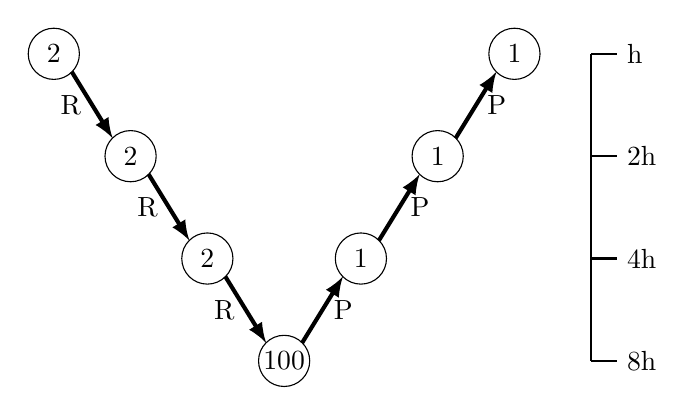
\begin{tikzpicture}[scale=0.65]
        \draw (0,8) circle (0.5) node {2};
        \draw (1.5,6) circle (0.5) node {2};
        \draw (3,4) circle (0.5) node {2};
        \draw (4.5,2) circle (0.5) node {100};
        \draw (6,4) circle (0.5) node {1};
        \draw (7.5,6) circle (0.5) node {1};
        \draw (9,8) circle (0.5) node {1};
        \draw[->, thick, >=latex, line width=1.5pt] (0.35,7.65) -- (1.15,6.35) node[midway,left] {R};
        \draw[->, thick, >=latex, line width=1.5pt] (1.85,5.65) -- (2.65,4.35) node[midway,left] {R};
        \draw[->, thick, >=latex, line width=1.5pt] (3.35,3.65) -- (4.15,2.35) node[midway,left] {R};
        \draw[->, thick, >=latex, line width=1.5pt] (7.85,6.35) -- (8.65,7.65) node[midway,right] {P};
        \draw[->, thick, >=latex, line width=1.5pt] (6.35,4.35) -- (7.15,5.65) node[midway,right] {P};
        \draw[->, thick, >=latex, line width=1.5pt] (4.85,2.35) -- (5.65,3.65) node[midway,right] {P};
        \draw[thick] (10.5,8) -- (10.5,2);
        \draw[thick] (10.5,8) -- (11,8) node[right] {h};
        \draw[thick] (10.5,6) -- (11,6) node[right] {2h};
        \draw[thick] (10.5,4) -- (11,4) node[right] {4h};
        \draw[thick] (10.5,2) -- (11,2) node[right] {8h};
    \end{tikzpicture}
    % \fadaptada{rogenski2011desenvolvimento}
\end{figure}
\end{frame}

%%%%%%%%%%%%%%%%%%%%%%%%%%%%%%%%%%%%%%%%%%%%%%%%%%%%%%%%%%%%%%
\subsection{Filtragem espacial}
%%%%%%%%%%%%%%%%%%%%%%%%%%%%%%%%%%%%%%%%%%%%%%%%%%%%%%%%%%%%%%

%%%%%%%%%%%%%%%%%%%%%%%%%%%%%%%%%%%%%%%%%%%%%%%%%%%%%%%%%%%%%%
\begin{frame}{Filtragem espacial}
\footnotesize{
\begin{align}
\left[\begin{array}{ccccccccccc}
1 &  & & & & & & & & &\\
 & 1 &  & & & & & & & & \\
& & 1 & & & & & & & &\\
& &  & . & . & .&  &  & & & \\
& & &  & \alpha & 1 & \alpha &  & & &  \\
& & & &  & . & . & . &  & & \\
& & & & &  &  & & 1 & & \\
& & & & &  &  & & & 1 & \\
& & & & &  &  & & &  & 1
\end{array}\right] \left[\begin{array}{c}
\varphi_{z1} \\
\varphi_{z2}  \\
\varphi_{z3}  \\
 . \\
\varphi_{zi}  \\
 . \\
\varphi_{zimax-2} \\
\varphi_{zimax-1} \\
\varphi_{zimax} 
\end{array}\right] = \hspace{1cm} \nonumber\\ 
=\left[\begin{array}{c}
(15\varphi_{z1}^* +  4 \varphi_{z2}^* -  6 \varphi_{z3}^* +  4  \varphi_{z4}^*
 -         \varphi_{z5}^* ) / 16 \\
( \varphi_{z1}^* + 12\varphi_{z2}^*+  6\varphi_{z3}^* -  4 \varphi_{z4}^*
+         \varphi_{z5}^*) / 16\\
 (   - \varphi_{z1}^* +  4\varphi_{z2}^*
+ 10\varphi_{z3}^* +  4\varphi_{z4}^* - \varphi_{z5}^* ) / 16\\
. \\
\begin{gathered}
af \varphi_{z_i}^*+bf\left[\varphi_{z_{i+1}^*}+\varphi_{z_{i-1}^*}\right]+ \\
cf\left[\varphi_{z_{i+2}^*}+\varphi_{z_{i-2}^*}\right]+df\left[\varphi_{z_{i+3}^*}+\varphi_{z_{i-3}^*}\right]
\end{gathered} \\
. \\
( - \varphi_{zimax}^* +  4\varphi_{zimax-1}^* + 10\varphi_{zimax-2}^* +  4\varphi_{zimax-3}^* - \varphi_{zimax-4}^* ) / 16  \\
(\varphi_{zimax}^* + 12\varphi_{zimax-1}^* +  6\varphi_{zimax-2}^* -  4 \varphi_{zimax-3}^* + \varphi_{zimax-4}^*) / 16 \\
(15\varphi_{zimax}^* +  4\varphi_{zimax-1}^* -  6 \varphi_{zimax-2}^* +  4  \varphi_{zimax-3}^* -  \varphi_{zimax-4}^*)/16 \end{array}\right]\label{filtragem_espacial}
\end{align}}
\normalsize
\normalsize
\end{frame}

%%%%%%%%%%%%%%%%%%%%%%%%%%%%%%%%%%%%%%%%%%%%%%%%%%%%%%%%%%%%%%
\begin{frame}{Filtragem espacial}
\begin{itemize}
    \item Define-se também as constantes $af=(11+10\alpha)/16$, $bf=(15+34\alpha)/64$, $cf=(-3+6\alpha)/32$ e $df=(1-2\alpha)/64$ segundo \cite{lele1992compact};
    \item A filtragem é aplicada ao final de cada iteração temporal e consiste em recalcular a distribuição dos componentes de vorticidade por meio de um sistema; 
    \item O valor do $\alpha$ é escolhido de acordo com a faixa de frequências que se deseja filtrar.
\end{itemize}
\end{frame}

%%%%%%%%%%%%%%%%%%%%%%%%%%%%%%%%%%%%%%%%%%%%%%%%%%%%%%%%%%%%%%
\subsection{Calculo das condições de contorno}
%%%%%%%%%%%%%%%%%%%%%%%%%%%%%%%%%%%%%%%%%%%%%%%%%%%%%%%%%%%%%%

%%%%%%%%%%%%%%%%%%%%%%%%%%%%%%%%%%%%%%%%%%%%%%%%%%%%%%%%%%%%%%
\begin{frame}{Calculo das condições de contorno}
Na formulação Vorticidade-Função de Corrente, conforme apresentado por \cite{roache1972computational}, o cálculo da vorticidade é realizado após a determinação da função corrente $ \psi $. Utilizam-se aproximações de quarta ordem para obter maior precisão nas derivadas, conforme mostrado nas equações \eqref{parede_baixo_vortici} a \eqref{parede_direita_vortici}:
\begin{align}
    \omega_{i,1} &= \frac{-85\psi_{i,1} + 108\psi_{i,2} - 27\psi_{i,3} + 4\psi_{i,4}}{18dy^{2}} + O(h^{4}), \label{parede_baixo_vortici} \\
    \omega_{i,jmax} &= \frac{11u_{i,jmax} - 18u_{i,jmax-1} + 9u_{i,jmax-2} - 2u_{i,jmax-3}}{6dy} + O(h^{4}), \label{parede_cima_vortici}\\
    \omega_{1,j} &= \frac{-85\psi_{1,j} + 108\psi_{2,j} - 27\psi_{3,j} + 4\psi_{4,j}}{18dy^{2}} + O(h^{4}), \label{parede_esquerda_vortici}\\
    \omega_{imax,j} &= \frac{-85\psi_{imax,j} + 108\psi_{imax-1,j} - 27\psi_{imax-2,j} + 4\psi_{imax-3,j}}{18dy^{2}} + O(h^{4}). \label{parede_direita_vortici}
\end{align}
\end{frame}